% vim: set tw=78 sts=2 sw=2 ts=8 aw et ai:
\documentclass[conference]{IEEEtran}

\usepackage{ucs}
\usepackage[utf8x]{inputenc}
\usepackage[english]{babel}
%\usepackage{hyperref}	  % use \url{http://$URL} or \href{http://$URL}{Name}
\usepackage{underscore}	  % underscores need not be escaped
\usepackage{subfigure}
\usepackage{verbatim}
\usepackage{float}
\usepackage{amsmath, amsthm, amssymb}

% Support for including graphics
\usepackage{graphicx}
\DeclareGraphicsExtensions{.pdf,.png,.jpg}

\usepackage[outerbars,color]{changebar}
\cbcolor{red}

\let\Oldcbstart\cbstart
\let\Oldcbend\cbend
%\renewcommand{\cbstart}{\color{red}\Oldcbstart}
%\renewcommand{\cbend}{\Oldcbend\color{black}}
\renewcommand{\cbstart}{}
\renewcommand{\cbend}{}

\begin{document}

\title{P2P-Tube: A Video Sharing Web Platform Based on Next-Share Technology}

\author{\IEEEauthorblockN{Călin-Andrei Burloiu}
\IEEEauthorblockA{Automatic Control and Computers Faculty\\
University Politehnica of Bucharest\\
Emails: calin.burloiu@gmail.com}}

\maketitle

\begin{abstract}
TODO ... a scalable video sharing web platform, named P2P-Tube. Part of the European project P2P-Next, our platform aims to be a complete web solution for the next generation video sharing technology, which is NextShare.
\end{abstract}

%\textbf{\textit{Keywords -- ala, bala, portocala}}

\begin{IEEEkeywords}
Video-On-Demand, NextShare, P2P-Next
\end{IEEEkeywords}

%\IEEEpeerreviewmaketitle

\section{Introduction}
\label{sec:introduction}
Since the emergence of the web the way applications are designed has changed. User interfaces are migrating to HTML-based solutions, in conjunction with CSS and JavaScript, for example Windows 8 will be based on HTML5 \cite{win8-html5}. More and more applications are migrating to the cloud being accessed thorough a web browser interface, for example Google Docs is a web-based alternative to the desktop Microsoft Office. Following this flow, communication protocols have also adhered to the new web paradigm, through the emergence of \textit{web services}, which implement communication on top of existing application protocols, like HTTP and its WWW protocol stack.

The main advantages of web services are interoperability and their small implementation overhead. Being built over standard protocols like HTTP, a lot of libraries already support it and the main communication primitives are already implemented. Thus developers do not need to handle this aspects and can focus on specific protocol requirements. In comparison, the standard approach of sending protocol messages directly over TCP or UDP, requires an additional development overhead every time basic communication primitives are being implemented.

Part of our work to the European project P2P-Next \cite{p2p-next} is P2P-Tube, a video sharing web platform for deploying sites like YouTube. P2P-Next goal is to build the next generation Peer-to-Peer content delivery platform. NextShare technology facilitates video streaming through BitTorrent and peer-to-peer protocols. Users are able to download video content not only from a number of delivery servers, which assume the role of \textit{seeders}, but also concomitantly from other users, which are \textit{leechers}. P2P-Tube platform uses this technologies in a set of browser plugins which are capable of providing video-on-demand and live streaming.

Applications built on top of P2P-Tube, need to offer users the possibility of uploading new videos. In order to make the application scale to a large amount of users which are concurrently doing this, we have designed a distributed system which uses one or more Content Ingestion Servers (CIS). Their role is to prepare uploaded videos for sharing with other users and make those videos available on the platform. We have chosen web services as the way of communication between web servers, which deliver the P2P-Tube application to the users, and Content Ingestion Servers.

In Section \ref{sec:web-services} we present state of the art solutions for web services. Section \ref{sec:security-solutions} introduces ways to secure those web services. P2P-Tube platform is presented in Section \ref{sec:p2p-tube} and implementation of security into CIS in Section \ref{sec:implementation}. An analysis of the reasons behind our choice for a particular web service technology and a particular security solution is also presented here. We conclude this article in Section \ref{sec:conclusion}.

\section{P2P-Next's Next-Share Technology}
\label{sec:next-share}
P2P-Next is an FP7 European project made up by a consortium of academic and industrial players which aim to build the next generation \textit{peer-to-peer (P2P)} content delivery platform. 21 partners from 12 different countries are involved here: BBC, Technische Universiteit Delft, Pioneer, Technical Research Center of Finland and also University Politehnica of Bucharest, were P2P-Tube platform was developed. P2P-Next takes as design principals the usage of open standards, open source development and future proof iterative integration.

In the last ten years two emerging trends sparkled the evolution of Internet: first of all more and more users share their content through social networks and P2P systems and secondly video sharing, video-on-demand and live streaming are increasingly gaining popularity. The current Internet infrastructure was not initially designed for simultaneous transmission of live events to millions of people and proposed technologies like multicasting do not seem to solve the problem. Television is no longer the main medium for audio and visual information content. Motivated by all these facts, P2P-Next started research and development of a new multimedia infrastructure based on both P2P technologies like BitTorrent and video streaming.

Next-Share is the name of the content delivery technology provided by P2P-Next which enables features such as on-demand video and live video for both computers and STBs (digital set-top-boxes) usable with TVs. Its main advantage against a classical video streaming technology is that the overhead of the video stream provider is diminished. Part of the computational and network resources are taken by each consuming peer from the system.

Next-Share platform implements its core functionality into NextShareCore which is written in Python. Video rendering in a PC browser using Next-Share can be done with two types of plugins: SwarmPlayer and NextSharePC.

A de facto standard today for playing videos in a browser is Adobe Flash Player. Because this is a proprietary technology and P2P-Next uses open standards, other technologies needed to be explored. W3C (World Wide Web Consortium) currently works at a new version of HTML, HTML5, which supports, besides other revolutionary features, audio and video tags. Thus video files can be easily embedded into web pages, just like images, without any browser extensions or plugins. Although HTML5 is still a draft, most modern browsers already implement some of its features including video and audio tags. On this background, non-profit organizations and big corporations have engaged in a codec war. Some of the problems were whether to accept or not proprietary codecs, which codecs should standardly accepted etc.. For instance Microsoft promotes AVC / H.264, a proprietary video codec. Despite of its image quality and its good compression ratio, non-profit organizations criticized it for being proprietary and closed standard. As a consequence Ogg containers with Vorbis audio codec and Theora video codec were included into HTML5. Google also stepped into this war and acquired On2 Technologies, for VP8, an open video compression format. They proposed WebM containers with Vorbis audio compression and VP8 video compression. Because Google's proposal is a free open standard it was accepted into HTML5 along with Ogg (Vorbis + Theora). Currently most modern browsers support video tags with Ogg and WebM containers.

P2P-Next developed \textbf{SwarmPlayer}, a Next-Share compliant browser plugin which is based on HTML5. It is currently supported in Windows in Mozilla Firefox as an extension and in Internet Explorer and there is also a Mac version.

Because only a few video formats are supported in HTML5 and older browsers do not support HTML5 video tags P2P-Next developed another variant of its Next-Share plugin, named \textbf{NextSharePC}. This one is based on VLC Player libraries to render videos and is able to play a lot of video formats, basically anything that is supported by VLC Player. Written by the VideoLAN project, VLC Media Player is a free open source cross-platform multimedia player and framework. Its disadvantage is that it is currently supported only in Windows, for both Mozilla Firefox, as a plugin, and Internet Explorer.

A NextShare plugin consists of two major parts: the browser plugin / extension, running in the browser address space and the Next-Share Agent API which facilitates communication with the NextShareCore.

\section{Design Overview}
\label{sec:design}
Besides the need to incorporate Next-Share technologies, P2P-Tube was also designed to be useful to the users. In the next subsections the usability and technical needs that governed our architecture are explained.

\subsection{Design Principles}
\label{subsec:design-principles}

P2P-Tube platform has been designed with a few basic design principles in mind:

\begin{enumerate}
 \item Provide as much as possible the \textbf{features} needed by such a platform, as they appear on similar platforms from the web.
 \item Provide to users a familiar \textbf{user interface} which resembles similar platforms from the web.
 \item Ensure that the platform \textbf{scales} well to a size of a few thousands of users.
 \item Ensure that the platform is \textbf{general purpose}.
 \item Make the platform available for \textbf{free} and distribute the code as \textbf{open-source}, encouraging community contributions.
\end{enumerate}

Being developed in academia, in University Politehnica of Bucharest, P2P-Tube was designed to fit well to our needs. The scalability requirements of a few thousands users, enumerated in Principle 3 above is enough for our Faculty of Automatic Control and Computers. However, despite this product was designed in the academia and fits its needs, we ensure that it can be generally purpose as stated in Principle 4 because of the features incorporated and its user interface tied to Principles 1 and 2.

\subsection{Features}
\label{subsec:features}

P2P-Tube provides to the users the following features:

\begin{itemize}
 \item \textbf{Categories}. Video assets can be grouped in \textit{categories} for a better organization of them.
 \item \textbf{Video plugin switching}. If the user has installed both Next-Share plugins (NextSharePC and SwarmPlayer) he is able to switch between them at any moment from the video watching page.
 \item \textbf{Users and accounts}. Users can apply for an account by registering to the site. Throughout registration, several fields can be completed, some of them mandatory, some of them optional, defining the \textit{user profile}. Authentication is possible through three methods: \textit{internal authentication}, \textit{LDAP authentication} and \textit{OpenID authentication}.
 \item \textbf{Uploading video assets}. Logged in users can upload new video assets to the site, which can be seen by others.
 \item \textbf{Social interaction}. Users can see each other's profiles, comment each other's video assets and vote them. Video assets uploaded by an user can be explored.
 \item \textbf{Searching}. Video assets can be searched by keywords and the results must be ordered by their relevance. The search can be done in the whole set of videos or in a particular category.
\end{itemize}

\textit{Internal authentication} is for users that applied for an account by the \textit{Registration} page. There are situations when the platform must be integrated with other services or sites. For example in our university we use P2P-Tube to share videos of technical presentations, courses or social events. We also have Moodle learning platform where students already have an account, so it was desired that users can authenticate on P2P-Tube we the same account credentials from Moodle. This has been achieved thorough LDAP which permits students to authenticate on both sites with the same user name and password, without requiring them to create an additional account. Another way to make users skip signing up is by using OpenID, a standard protocol which allows them to sign in through an account from another site. However, this third party site must support OpenID. So, for example, users that already have an account on Yahoo!, Google, Twitter or WordPress can securely sign in with the same user names and passwords from that accounts. When users log in for the first time using external authentication, like LDAP or OpenID, they must complete their profile.

Users can upload video assets through an upload mechanism described in the next subsection.

\subsection{Content Ingestion}
\label{subsec:content-ingestion}

NextSharePC can play any video format as long as VLC supports it and SwarmPlayer supports only video containers and codecs which are compliant with HTML5. Most modern browsers support videos having Ogg containers with Vorbis audio compression and Theora video compression or WebM containers with Vorbis audio compression and VP8 video compression. Users must be able to upload videos in a format of their choice like MPEG, DivX or AVC/H.264. Thus, the platform must perform a conversion, also known as \textit{transcoding}, from an input user format to a NextShare compliant format. P2P-Tube converts all video assets to videos with Ogg containers and Vorbis+Theora compression in order to be compatible with most modern browsers and to make video assets playable with any of the two NextShare plugins. However this can be changed from the platform configuration.

Besides video transcoding, several other operations must be performed in order to make new video assets available on the platform. This is done by a \textbf{Content Ingestion Server} (\textbf{CIS}) which is typically located on a different machine.

An user uploads a video file, referred here as \textit{raw video file}, to a web server and may also provide additional information about it, like title, description, tags etc.. When video upload is finished the process of content ingestion is started by the web server by sending a content ingestion request to a CIS. This is done directly, if the system has a single CIS, or indirectly via a CIS Load Balancer (CIS-LB), which forwards the request to one CIS from a pool of several CIS machines. By doing load balancing, the indirect request method provides scalability because more content ingestion jobs can run in parallel, allowing more users to add content simultaneously to the platform. By these means availability is also increased, the system becoming fault tolerant in case of CIS failures.

Note that sending content ingestion request is transparent for the web server. There is no difference for it if this is done directly to a CIS or indirectly through a CIS-LB. This simplifies implementation of the web server and hides the abstraction of content ingestion from it.

\begin{figure}[h]
  \begin{center}
    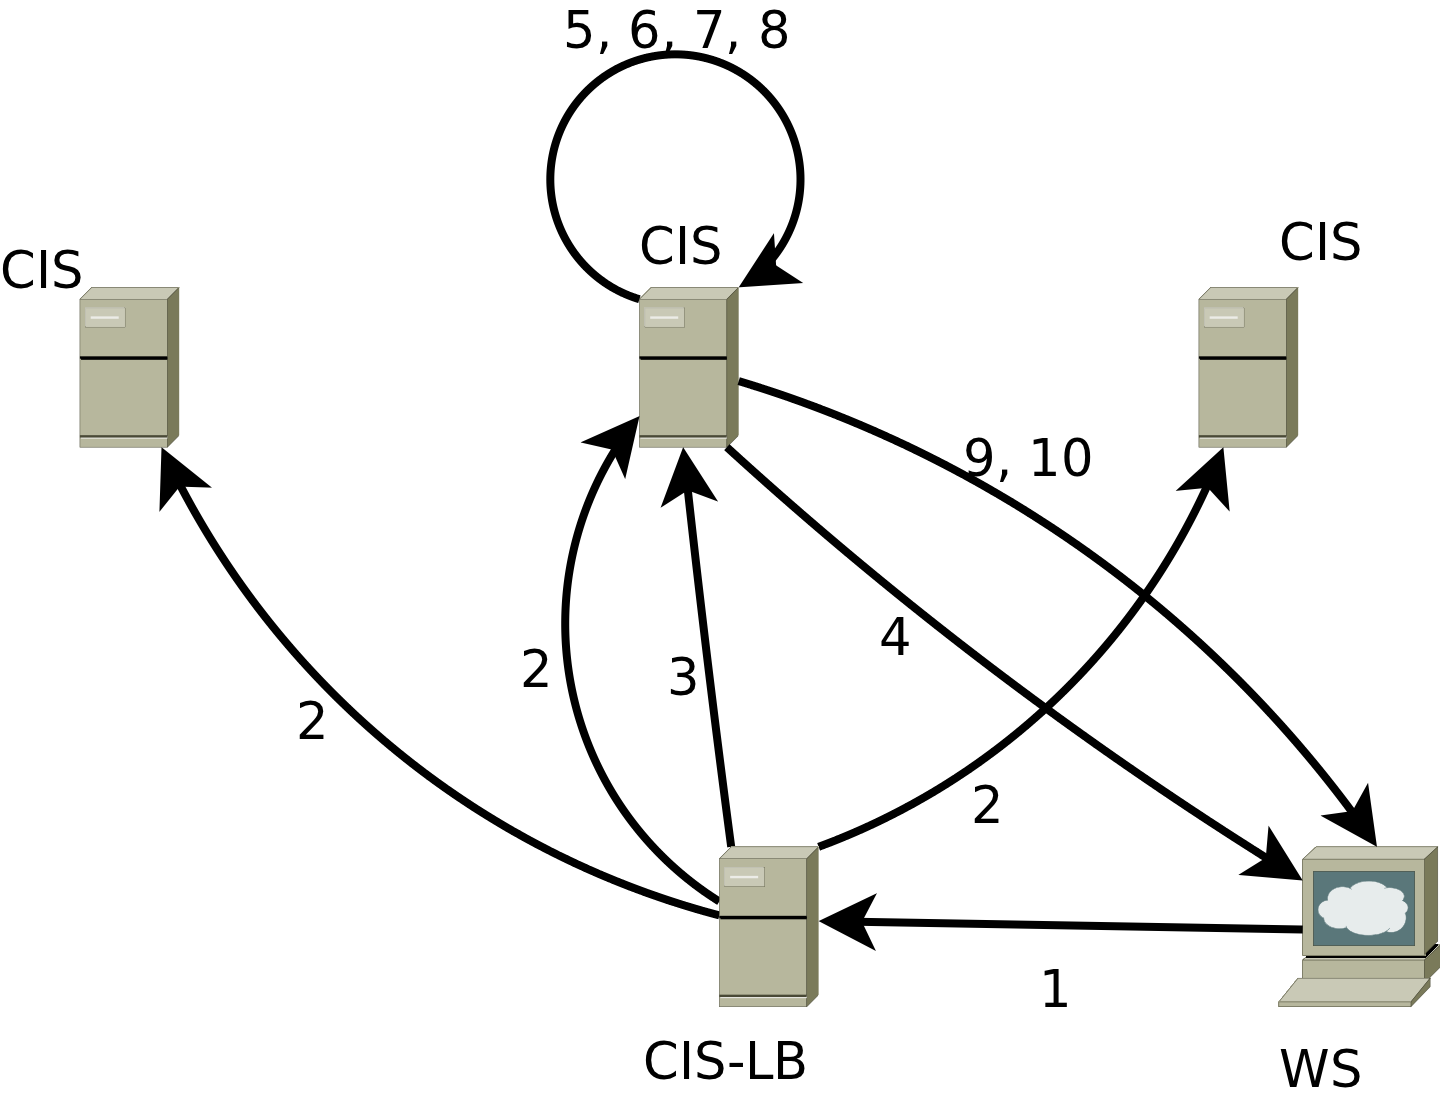
\includegraphics[width=\columnwidth]{img/content-ingestion.png}
  \end{center}
  \caption{Content Ingestion Process}
  \label{fig:content-ingestion}
\end{figure}

CIS operation through a CIS Load Balancer is described in Figure \ref{fig:content-ingestion}. Until the end of this subsection, the numbers in brackets refer to arrows from the figure. The web server sends a \textbf{content ingestion request} to CIS-LB (1), which must choose the least loaded CIS from the system. To do this it queries each CIS for its load by sending a \textbf{get load request} (2) and establishes by processing the answer which one is the least loaded. The content ingestion request previously received is then forwarded to the least loaded CIS (3), informing it about the new video file that has been uploaded. The message also contains information about one or more formats in which the video must be converted referred here as \textit{destination formats}. This information includes parameters for each format like image resolution, frame rate, audio quality etc.. The least loaded CIS which received the request executes a job on the uploaded raw video file by doing the following operations:

\begin{itemize}
 \item \textbf{Transfers locally} (4) the raw video file from the web server.
 \item \textbf{Transcodes} (5) the raw video file to one or more \textit{destination formats} resulting \textit{transcoded video files}.
 \item \textbf{Extracts image thumbnails} (6) from the raw video file.
 \item \textbf{Creates torrent files} (7) (\textit{.tstream}) for transcoded video files.
 \item \textbf{Seeds} (8) the transcoded video files by using the torrent files previously created.
 \item \textbf{Transfers back} (9) torrent files and image thumbnails to the web server.
 \item Notifies the Web Server about the \textbf{job completion} (10) so that it can make the video accessible to the users.
\end{itemize}

In the end of the content ingestion process all other Content Ingestion Servers from the system must be aware of the new torrent files in order to seed them. First of all, the new torrent files need to be locally accessible to them, so all torrent files can be shared by CIS machines on a \textit{distributed file system} such as NFS, LustreFS or GlusterFS. The overhead of using shared storage between CIS machines shouldn't affect performance, even if NFS is used, which serves files through a single machine. This is because torrent files are very small so concurrently accessing more files on the shared file system can affect performance in a negligible manner.

When the web server is notified about the job completion (10) a seed request must arrive to each CIS so that they can start seeding the new torrent files available in the distributed file system. This request is originated from the web server and there is no need to do this on a single CIS system, because this is already done in step 8 from Figure \ref{fig:content-ingestion}, so the web server can be configured to skip this redundant step from its configuration. In a multiple CIS system this step is mandatory for ensuring high availability of the new video assets. Thus, a \textbf{seed request} is sent from web server to CIS-LB, which forwards this message to all CIS from its jurisdiction. Upon reception they will start seeding requested torrent files which are located in the distributed file system.

\section{Implementation}
\label{sec:implementation}
One of the basic design principles of our platform was to publish it as open-source encouraging community contributions. To facilitate this we have chosen popular programming languages, frameworks and technologies in order to better attract open-source communities around our platform. These decisions along with implementation details are given in this section. Information found here accompanied by comments from the source code should hopefully provide enough information to a new contributor to this project.

Our implementation was designed to work on \textbf{GNU/Linux} distributions, so our back end dependencies, such as FFmpeg, has been chosen based on this. However we tried as much as possible to choose them such that they also run on other operating systems, such as Windows. Thus, porting P2P-Tube for them should be easy, but until this point creating a cross-platform implementation was not a priority for us.

\subsection{Web Application Front End}
\label{subsec:front-end}

The front end of P2P-Tube provides an interface with the users of the platform. Today more and more applications are migrating from a classical desktop interface to a web interface. For instance, applications like Microsoft Office started to appear on the cloud, providing a web interface; one popular example is Google Docs. Besides this new trend, Next-Share content delivery platform was successfully implemented in browsers by P2P-Next. So implementing P2P-Tube as a web platform came as a natural choice.

Because almost any hosting provider offers a standard LAMP stack, we decided to cope with such a configuration. LAMP stands for Linux, Apache, MySQL, PHP, the technologies which is based on. We tested P2P-Tube on Apache web server, but it should work well on others.

P2P-Tube server side application is implemented in \textbf{PHP} which is one of the most popular programming languages for this purpose. To facilitate development we decided to use \textbf{CodeIgniter} \cite{code-igniter} open-source framework. Thanks to this framework the platform uses a \textit{MVC (Model-View-Controller)} design pattern, which separates the user interface part (View), from the data stored (Model) under the rule of the Controller.

Our implementation uses a \textbf{MySQL} database, but CodeIgniter abstracts the interface with the database, so porting our platform for a different SQL technology such as PostgreSQL should be easy.

As a web application, on the client side P2P-Tube uses HTML, CSS and JavaScript. As stated before SwarmPlayer only works with browsers that support HTML5. We decided to use jQuery \cite{jquery} as a JavaScript framework to ease development on the client side programming. We developed a jQueryUI \cite{jqueryui} widget which is used to control video playing with features like play, pause and stop buttons, time progress slider, volume control etc.. This widget is detailed in Subsection \ref{subsec:video-widget}.

The web application currently uses two models. \textbf{\texttt{videos} model} is an interface to the database for accessing information about video assets. \texttt{videos} table contains on each row data about a video asset. \texttt{videos_comments} stores each video comment created by an user on a row. Both videos and comments can be voted with like or dislike. Methods for returning detailed information about a video, for returning \textit{video summaries} and for searching in the videos set are implemented here. Video summaries are lists of video assets, with brief information about each one. For instance, \texttt{get_videos_summary} method can create a list of videos from a specific category, uploaded by a specific user, within a defined range described as offset and count and ordered in a specific way. Methods for adding and retrieving comments for voting or for incrementing the number of views for a video are also available here.

\textbf{\texttt{users} model} is an interface to the database for accessing information about users. \texttt{users} table stores on each row data about a registered user, including its user name, its password SHA1 hash, its e-mail and profile information such as gender, country, city, birth date etc.. Authentication information, authentication method (internal, with LDAP or with OpenID) and user preferences are also stored in this table. When signing in with OpenID, \texttt{users} table is joined with \texttt{users_openid} table which maps OpenID URLs with rows from \texttt{users} table. After registration, new users have to confirm their e-mail address by providing an activation code received on that address. Unactivated users with their activation codes are stored in \texttt{users_unactivated}. User activity is logged in \texttt{users_actions} table. This kind of information can be used to ensure that an user votes a comment or a video only one time during a day, but user history can also be tracked here.

\texttt{users} model methods can be used to check authentication credentials, to register new users, to activate accounts, to send password recovery e-mails and to modify user data. Column \texttt{auth_src} from \texttt{users} table identifies the authentication method used by the user. If internal authentication is used the password entered by the user is hashed with SHA1 and checked against the hash from \texttt{password} column. For LDAP authentication this field is NULL, because \texttt{users} model connects to an LDAP server for logging in. For authentication through OpenID, \texttt{users} model uses a third-party library developed by JanRain Inc. \cite{janrain-openid} which implements OpenID protocol.

Pages are organized around a few controller classes. \textbf{\texttt{catalog} controller} manages web pages that help users explore video assets. \textbf{Index page} shows the five most \textit{hottest} video assets from each category which are the newest and the most appreciated ones. The appreciation score is calculated as the number of views plus the number of likes minus the number of dislikes, so a video with a greater appreciation score is more appreciated. \textbf{Category page} permits users to explore video assets by category. Videos can be ordered alphabetically, by upload date or by showing the hottest first.

\textbf{\texttt{video} controller} manages the \textbf{watch page} were users can play a video asset with one of the two Next-Share plugins and the video widget presented in Subsection \ref{subsec:video-widget}. Commenting and voting mechanisms are also implemented into this controller through AJAX, such that when using this facilities the web page is not refreshed interrupting video playing.

\textbf{\texttt{user} controller} is used for user management. \textbf{\texttt{login} method} controls a web page which permits users to sign in with their user name and password or by providing an OpenID. Tree buttons for Yahoo!, Google and myOpenID ease authentication through OpenID with this services. \texttt{login} method checks authentication credentials by using \texttt{users} model and sets a new session in a cookie if authentication succeeded. To delete the session and sign out, \texttt{logout} method is used. \textbf{Registration} and account activation pages are managed by the same controller and logged in users can access \textbf{account page} to change account and profile information or to change their password. To verify that a real person applied for an account, a CAPTCHA is provided on the registration page. Users can see each other's profile through the \textbf{profile page} where one can also see what videos that user uploaded.

The platform provides a way to load static HTML as page content through \textbf{\texttt{article} controller}. The HTML is loaded from \textit{``application/views/article/$<$language$>$/$<$article_name$>$.php''} when URL \textit{``article/$<$article_name$>$''} is accessed. \textit{$<$language$>$} is the name of the current language set in \textit{``application/config/config.php''}. CodeIgniter's URI routing feature can be used in order to have a different URL for an article. In the default configuration of the P2P-Tube site there are four articles used: \textit{Install Plugins}, \textit{About}, \textit{Help} and \textit{Contact}. All of them use URI Routing in order to have a friendlier address.

CodeIgniter supports running its script from the command line. \textbf{\texttt{admin_cli} controller} implements a few methods that can be used by system administrators exclusively from the command line. Database cleanup methods are currently implemented here, which can be conveniently called as cron jobs.

Some parts of a web page are common to more than one page. This include headers, menus, footers, side parts with optional information etc.. All these components are implemented as \textbf{views} and are loaded within the controller of each page. \textbf{\texttt{header} view} renders the top of a web page and includes a menu, a logo, information about the logged in user if required and a search box that help users search video assets, described in Subsection \ref{subsec:searching}. \textbf{\texttt{footer} view} renders the bottom of a web page and typically contains copyright information or links. Common HTML tags like those found into head tag can be easily loaded by using views \textbf{\texttt{html_begin}} and \textbf{\texttt{html_end}}. View \texttt{html_begin} is used with \textbf{\texttt{Html_head_params} library} to load CSS files, JavaScript files, set the page title and add meta data.

\subsection{Searching Video Assets}
\label{subsec:searching}

\subsection{Video Widget}
\label{subsec:video-widget}

TODO

\subsection{Content Ingestion Back End}
\label{subsec:back-end}

TODO

\subsection{Front End and Back End Communication}
\label{subsec:communication}

The web server needs to communicate with Content Ingestion Server, whether or not through a CIS Load Balancer (CIS-LB), by sending a content ingestion request. By using a web service for this communication the implementation overhead is reduced. Sending HTTP requests from the PHP web server application is much more easy then creating a custom new protocol. The same applies at the other communication point, the Python server, where requests are received by Web.py framework, which makes HTTP methods processing extremely easy.

If another framework decides to use our solution based on CIS machines, interoperability is simplified by using web service interfaces, no matter what programming language is used for web server application.

\subsection{Programming Languages, Frameworks}
\label{subsec:langs-and-frameworks}

Content Ingestion Server is written in Python, mainly because of the need of using threads. A master thread takes the role of a producer by receiving requests from clients and submitting them to a job queue. The consumer is a worker thread which gets jobs from the queue and executes them, using a first-come first-server servicing policy. If the queue is empty the worker waits without blocking until a new job is available. Client requests are received by the master with the aid of Web.py, a lightweight web framework \cite{webpy}.

\subsection{The Choice for the Web Service}
\label{subsec:securing-cis}

Our choice between a SOAP web service and a simple RESTful web service was based on our needs. We wanted to make a server with a low communication overhead and SOAP has the disadvantage of consuming more computational resources when processing requests. Our messages that need to be passed through different services have a simple structure. 

The \textit{get load request} does not have any parameters, so a simple HTTP GET request is sufficient and any extra data transmitted as XML with SOAP is redundant.

\textit{Content ingestion request} is a message with a greater complexity. The name of the uploaded file located on the web server needs to be transmitted, along with video formats information such as containers, codecs used, resolutions, frame rates, aspect ratios, audio sampling rates and bit rates. All these information would fit well as parameters in a SOAP message. However encoding then in a JSON seemed to be a much simpler solution. Both PHP and Python offer functions that convert their primitive types and data structures, like lists and dictionaries, into JSON strings. XML messages have a greater verbosity comparing to JSON messages. Features like XML tag attributes are not required for our application.

We expect web servers and their CIS Load Balancers to know CIS peers in advance. So there is no need for discovery services that could provide contact information for new CIS peers. This would reduce administrative control and would raise security concerns like discovering malicious CIS peers. So there is no need for service discovery features like UDDI from SOAP ecosystem.

Services functionality does not need to be described because it is expected to be known in advance by the client application, so SOAP's WSDL feature is not needed.

The simplicity of our web services and our need for a low communication footprint suggest us to use a RESTful web service with JSON encoded information when the POST method is needed. SOAP extra features like WSDL and UDDI are not required for our application, giving us another reason to exclude it as a candidate.

\subsection{Securing Content Ingestion Server}
\label{subsec:securing-cis}

As pointed in the previous section, we require a low communication overhead. In Section \ref{subsec:ws-sec-perf} we have shown that WS-Security needs more processing time for message parsing. But is this worth it?

WS-Security offers end-to-end security, but P2P-Tube web servers and CIS peers are designed to be tightly coupled, usually being in the same data center or under the authority of the same organization. All these components communicate directly without proxies. So a simple point-to-point communication over HTTPS could be enough for our application.

The additional overhead of WS-Security against TLS/SSL solution is a price to pay for the advantage of an end-to-end communication. However, our solution is not designed to use proxies. So HTTPS with TLS or SSL is enough for our application and is much more easy to implement. Usually any library that supports HTTP also supports HTTPS. On the server side two additional informations need to be passed: server's certificate and its private key.

Because CIS communication with a CIS-LB or with a web server can be encrypted, authentication information can be added into messages when using the HTTP POST methods. CIS requires an user name and a password for content ingestion requests.

If CIS, CIS-LB and web server peers are located in the same data center which is secured and isolated from the exterior, secure communication between them might not be required. Taking into account the fact that HTTPS doubles communication overhead, the system administrator must think twice before securing services' communication.

File transfer between web server and CIS is made through a pluggable interface. Other protocols like FTP \cite{ftp}, scp \cite{scp} and rsync \cite{rsync} can be used. We currently implemented an FTP interface, where the control channel is encrypted using TLS. Data channel does not require encryption if the files are not secret. Securing this channel would substantially increase resource usage. We are planning to implement a rsync file transfer interface too. This protocol is secured by default because is built over SSH. It also has the advantage of reducing the amount of data sent over the network by transferring only the differences between files. 



\section{Future Work}
\label{sec:future-work}
Our video-sharing platform is far from being a complete one, so we are planning to extend it in the following directions:

\begin{itemize}
 \item \textbf{Administration Interface}: the platform must have an advanced administration interface, where features, the user interface and moderation can be easily managed via a web interface. With moderation system administrators can ban users, delete video etc.. The general purpose open-source platform Joomla for example provides an administrion interface.
 \item \textbf{Video Support}: extending P2P-Tube to support other video technologies besides Next-Share. Normal HTML5 and VLC support and also Adobe Flash Player support without P2P streaming must be considered.
 \item \textbf{Swift Support}: P2P-Tube was designed to work with Next-Share by using BitTorrent protocol. Another better protocol that can be used is \textit{swift} \cite{swift}, which is currently an IETF draft.
 \item \textbf{Hierarchical Categories}: categories are currently defined as a list. In the future they should have a tree structure with categories, subcategories, subsubcategories etc..
 \item \textbf{Better language support}: currently our platform supports multiple languages with the native support from CodeIgniter and with article controllers language support. A better support would allow users to change the language directly from a P2P-Tube site. Also automatic language detection should be considered by locating the IP address of the user or by inferring it from the URL. For example, http://www.example.com/fr/page should use French, http://example.ro/ should be in Romanian and http://it.example.org/page should be in Italian. The current language should be reflected in the currect URL as in the previous examples such that search engines can also detect it, providing SEO (Search Engine Optimization).
 \item \textbf{Better Search Feature}: changing the current implementation of the search mechanism which is based on MySQL Full-Text with a more powerful one, such as one based on Apache Lucene or Apache Solr.
 \item \textbf{Porting for Other Operating Systems}: P2P-Tube should be ported for Windows Server.
 \item \textbf{Alternative Features for CIS}: file transfers should be supported with other more reliable protocols such as rsync and other tools for transcoding and thumbnail extraction should be considered.
 \item \textbf{Adapting CIS for Other Video Technologies}: if the platform includes normal support for HTML5, VLC, Adobe Flash or other technologies, CIS must be modified. One good reason could be that other technologies do not need seeding and creating torrents.
\end{itemize}


\section{Conclusion}
\label{sec:conclusion}
TODO

The web service solution to use depends a lot on the application requirements. Whether communication footprint is vital? Whether the service needs to published through a discovery service or not? Whether the service functionality needs to be described for other services or clients? For our application a RESTful web service best fitted, mainly because of our protocol simplicity and our need for a low communication overhead. Also a discovery feature was not required.

WS-Security offers a lot of features in comparison with HTTPS with TLS/SSL, like end-to-end communication and message integrity. If this are not required then HTTPS offers a lower overhead and is recommended to be used.

\section*{Acknowledgment}
\label{sec:acknowledgment}

Special thanks go to the P2P-Next~\cite{p2p-next} team who is working
enthusiastically to deliver the next generation peer-to-peer content delivery
platform. Their dedication, professionalism and vision are a constant factor
of motivation and focus for our work.

\bibliographystyle{abbrv}
\bibliography{p2p-tube}

\end{document}
